\documentclass[mscthesis]{usiinfthesis}
\usepackage{lipsum}

\usepackage[linesnumbered,nosemicolon,noline]{algorithm2e}
\usepackage{algpseudocode}
\usepackage{environ}

%For substeps in algo environment
\newcounter{parentAlgoLine}
\SetKwBlock{BEGIN}{}{}

\makeatletter
\NewEnviron{substeps}{%
  \refstepcounter{AlgoLine}% <---- remove if necessary
  \protected@edef\theparentequation{\theequation}%
  \setcounter{parentAlgoLine}{\value{AlgoLine}}%
  \setcounter{AlgoLine}{0}%
  \def\theAlgoLine{\theparentAlgoLine.\arabic{AlgoLine}}%
  \BEGIN{\BODY}%
  \setcounter{AlgoLine}{\value{parentAlgoLine}}%
  \ignorespacesafterend
}
\makeatother

%For algo sub-state

\newcounter{algsubstate}
\renewcommand{\thealgsubstate}{\alph{algsubstate}}
\newenvironment{algsubstates}
  {\setcounter{algsubstate}{0}%
   \renewcommand{\State}{%
     \stepcounter{algsubstate}%
     \Statex {\footnotesize\thealgsubstate:}\space}}
  {}

\usepackage{listings}
\graphicspath{ {./figures/} }

\lstdefinelanguage{algebra}
{morekeywords={import,sort,constructors,observers,transformers,axioms,if,
else,end},
sensitive=false,
morecomment=[l]{//s},
}

% Variables
%\newcommand\numberevents{61751 } % whole dataset
%\newcommand\numberevents{36013 } % number of invasions from 1850 to 2010
%\newcommand\numbereventsfilter{10840 } % number of invasions from 1850 to 2010

% For equations float
\usepackage{float}
\usepackage{aliascnt}
\newaliascnt{eqfloat}{equation}
\newfloat{eqfloat}{h}{eqflts}
\floatname{eqfloat}{Equation}

\newcommand*{\ORGeqfloat}{}
\let\ORGeqfloat\eqfloat
\def\eqfloat{%
  \let\ORIGINALcaption\caption
  \def\caption{%
    \addtocounter{equation}{-1}%
    \ORIGINALcaption
  }%
  \ORGeqfloat
}


\title{Alien species modelling via relational event models} %compulsory
%\specialization{Dependable Distributed Systems}%optional
%\subtitle{Subtitle: Reinventing the World} %optional 
\author{Niccol\`o Zuppichini} %compulsory
\begin{committee}
\advisor{Prof.}{Ernst-Jan Camiel}{Wit} %compulsory
\coadvisor{}{Igor}{Artico}{} %optional
\end{committee}
\Day{23} %compulsory
\Month{June} %compulsory
\Year{2022} %compulsory, put only the year
\place{Lugano} %compulsory

\dedication{To my beloved} %optional
\openepigraph{Hello there \dots}{General Kenobi} %optional

%\makeindex %optional, also comment out \theindex at the end

\begin{document}

\maketitle %generates the titlepage, this is FIXED
%TODO this causes problem...why?
\frontmatter %generates the frontmatter, this is FIXED

\begin{abstract}
%TODO mention the embedding of the process in a latent space
%TODO briefly report results
\newcommand\numberevents{36013 } % number of invasions from 1850 to 2010

% Topic introduction
During the last centuries, human research on the interaction of species substantially intensified. However, we know little to nothing about the underlying process that shapes the behaviors of alien species invasion across regions, countries, and ecosystems.

% What we do here
In this paper we present a relational event model to study the invasion of alien species, which are species found outside of their native region. We describe the invasion of species as a temporal unidirectional bipartite species-region graph. Under this framework, we present a relation event model to model the study of co-invasion of species. We then apply this model to a subset of the dataset of \numberevents events ranging from 1850 to 2010. The aim of this paper is hence to study what group of species has the tendency to co-invade a region.

% What we got
Using years of first records of \numberevents invasions of alien species from 17 taxonomic groups spanning from 1850 to 2010 we show how a custom relational event model can be used to model the dynamics of species invasion. Due to the high size of the dataset, we also present a high-performance implementation in python of our model.

\end{abstract}

%\begin{acknowledgements}
%\lipsum 
%\end{acknowledgements}

%\tableofcontents 
%\listoffigures %optional
%\listoftables %optional

\mainmatter

\chapter{Introduction}
% 1. Motivation. Why invasive species are a problem?
% 2. Briefly introduce the dataset
% 3. Briefly introduce how I will study the dataset
% 4. Briefly introduce how I will study the dataset
% 5. TODO briefly report the results

The rate at which alien species invade countries has increased over the last century and it is becoming an important issue. The economic impact of alien species in Europe is estimated to be close to 13 billion dollars annually (\cite{intro:rate}). The interest in the study of the dynamics of alien species has been increasing over the years for this reason. Unfortunately, due to the complexity of the problem, is hard to come up with real actions. Intuitively, the invasion rate of species differs belonging to different taxonomic groups, however, a comprehensive global invasion dynamics study of the last centuries subdivided by taxonomic groups is still lacking. The dynamics of invasive species are driven by a multitude of factors simultaneously. These factors can be complex involving exogenous, endogenous, sociological, ecological, and socio-economic factors. (\cite{intro:factors}). Given the complexity of the subject, it's important to develop a framework capable of studying and analyzing all the underlying effects simultaneously. 

Relational event modeling was first developed in the field of social network analysis (\cite{rem:butts}). A relational event is an interaction between a sender and a receiver at a specific timestamp. A relational event model studies the temporal sequence of such relational events. This framework has many advantages in the fact that it is able to study underlying temporal patterns, can efficiently deal with time-varying variables and it's an extremely adaptable hypothesis testing tool. Due to its versatility, in the years it is been applied in a large number of different fields such as animal-animal interaction (\citet{intro:cattle}), 
%TODO cite 2 more.

%%TODO what did other people do?
%In the years, there have been a large number of different statistical approaches to relation event models to predict the appearance and spread of alien species.  
%
%%TODO review this
%To tackle the problem a dataset containing an extensive amount of invasive species in multiple geographic regions worldwide.  has been created (\citet{intro:dataset}). To further extend this study \citet{intro:ecological} fitted a REM on the dataset. \\
%%TODO I can't find the "Analysing ecological dynamics with relational event
%%models: the case of invasion events" paper


In this thesis, we introduce a novel custom latent space relational event model to study the dynamics of co-invasion of species for a bipartite graph. The model takes into consideration multiple species simultaneously and studies the underlying relationship between different species co-invading regions by training on the most exhaustive source of first records of alien species in multiple regions in the world. Traditional statistical tools, such as multidimensional scaling, fail to capture the similarity of nodes on this dataset due to its bipartite nature (i.e. no interaction of the kind species-species and region-region). We propose a different approach to the study of this dataset by disposing the species and regions into a latent space and fitting a custom relational event model. By studying the proximity of species and regions in the latent space, our model is capable of determining the group of species that tend to co-invade a region and, in an analogous way, the group of regions that are more likely to be invaded by the same group of species.

%TODO briefly report the results

% Structure of the thesis
In chapter 2 we make a preliminary study of the dataset of the alien species and discuss previous research. In chapter 3 we present an exhaustive statistical background of the methods used for the reader. In chapter 4 we provide a formulation of our latent space relational event model and propose an efficient algorithm to make inferences about the latent space. In chapter 5 we report our results. In the conclusive chapter 6 we discuss our results.



\chapter{Materials and methods}
%TODO add some comments from the paper from the lady


The Alien Species First Records database \cite{intro:dataset} is the most exhaustive source of first records of alien species currently available. It contains the years of the first establishment of alien species in regions worldwide. 
The original dataset has been later updated to include a more depth invasion dataset \cite{intro:datasetv2} and is in continuously updated. The current version includes %TODO add numbers


\begin{table}[H]
\centering
\begin{tabular}{|l|l|l|l|l|}
\hline
Algae      & Birds       & Fishes        & Mammals  & Vascular plants \\ \hline
Amphibians & Bryophytes  & Fungi         & Molluscs & Viruses         \\ \hline
Arthropods & Bryozoa     & Insects       & Reptiles &                 \\ \hline
Bacteria   & Crustaceans & Invertebrates & Spiders  &                 \\ \hline             
\end{tabular}
\caption{The 19 taxonomic families.}
\label{table:families}
\end{table}

%TODO update the stats with the updated trimmed dataset
% By trimming the dataset, we removed 2495 relational events that happened before 1850. 
We focus our research on the time interval spanning from 1850 to 2010. The dataset we take into consideration includes 18 taxonomic (listed in Tab. \ref{table:families}) families and 276 regions \footnote{Regions generally correspond to countries but in the dataset available almost half regions are islands.}. Considering all taxonomic families there's a total of 19390 species. As Fig. \ref{fig:hist_tax_fam} shows, most of the species in the dataset lie in the "Vascular Plants" taxonomic family.
%Info right after import t = (1850, 2010)
%There are 18 families and 276 regions
%There are 19390 species.

\begin{figure}[H]
\centering
\begin{minipage}{.55\textwidth}
    \centering
    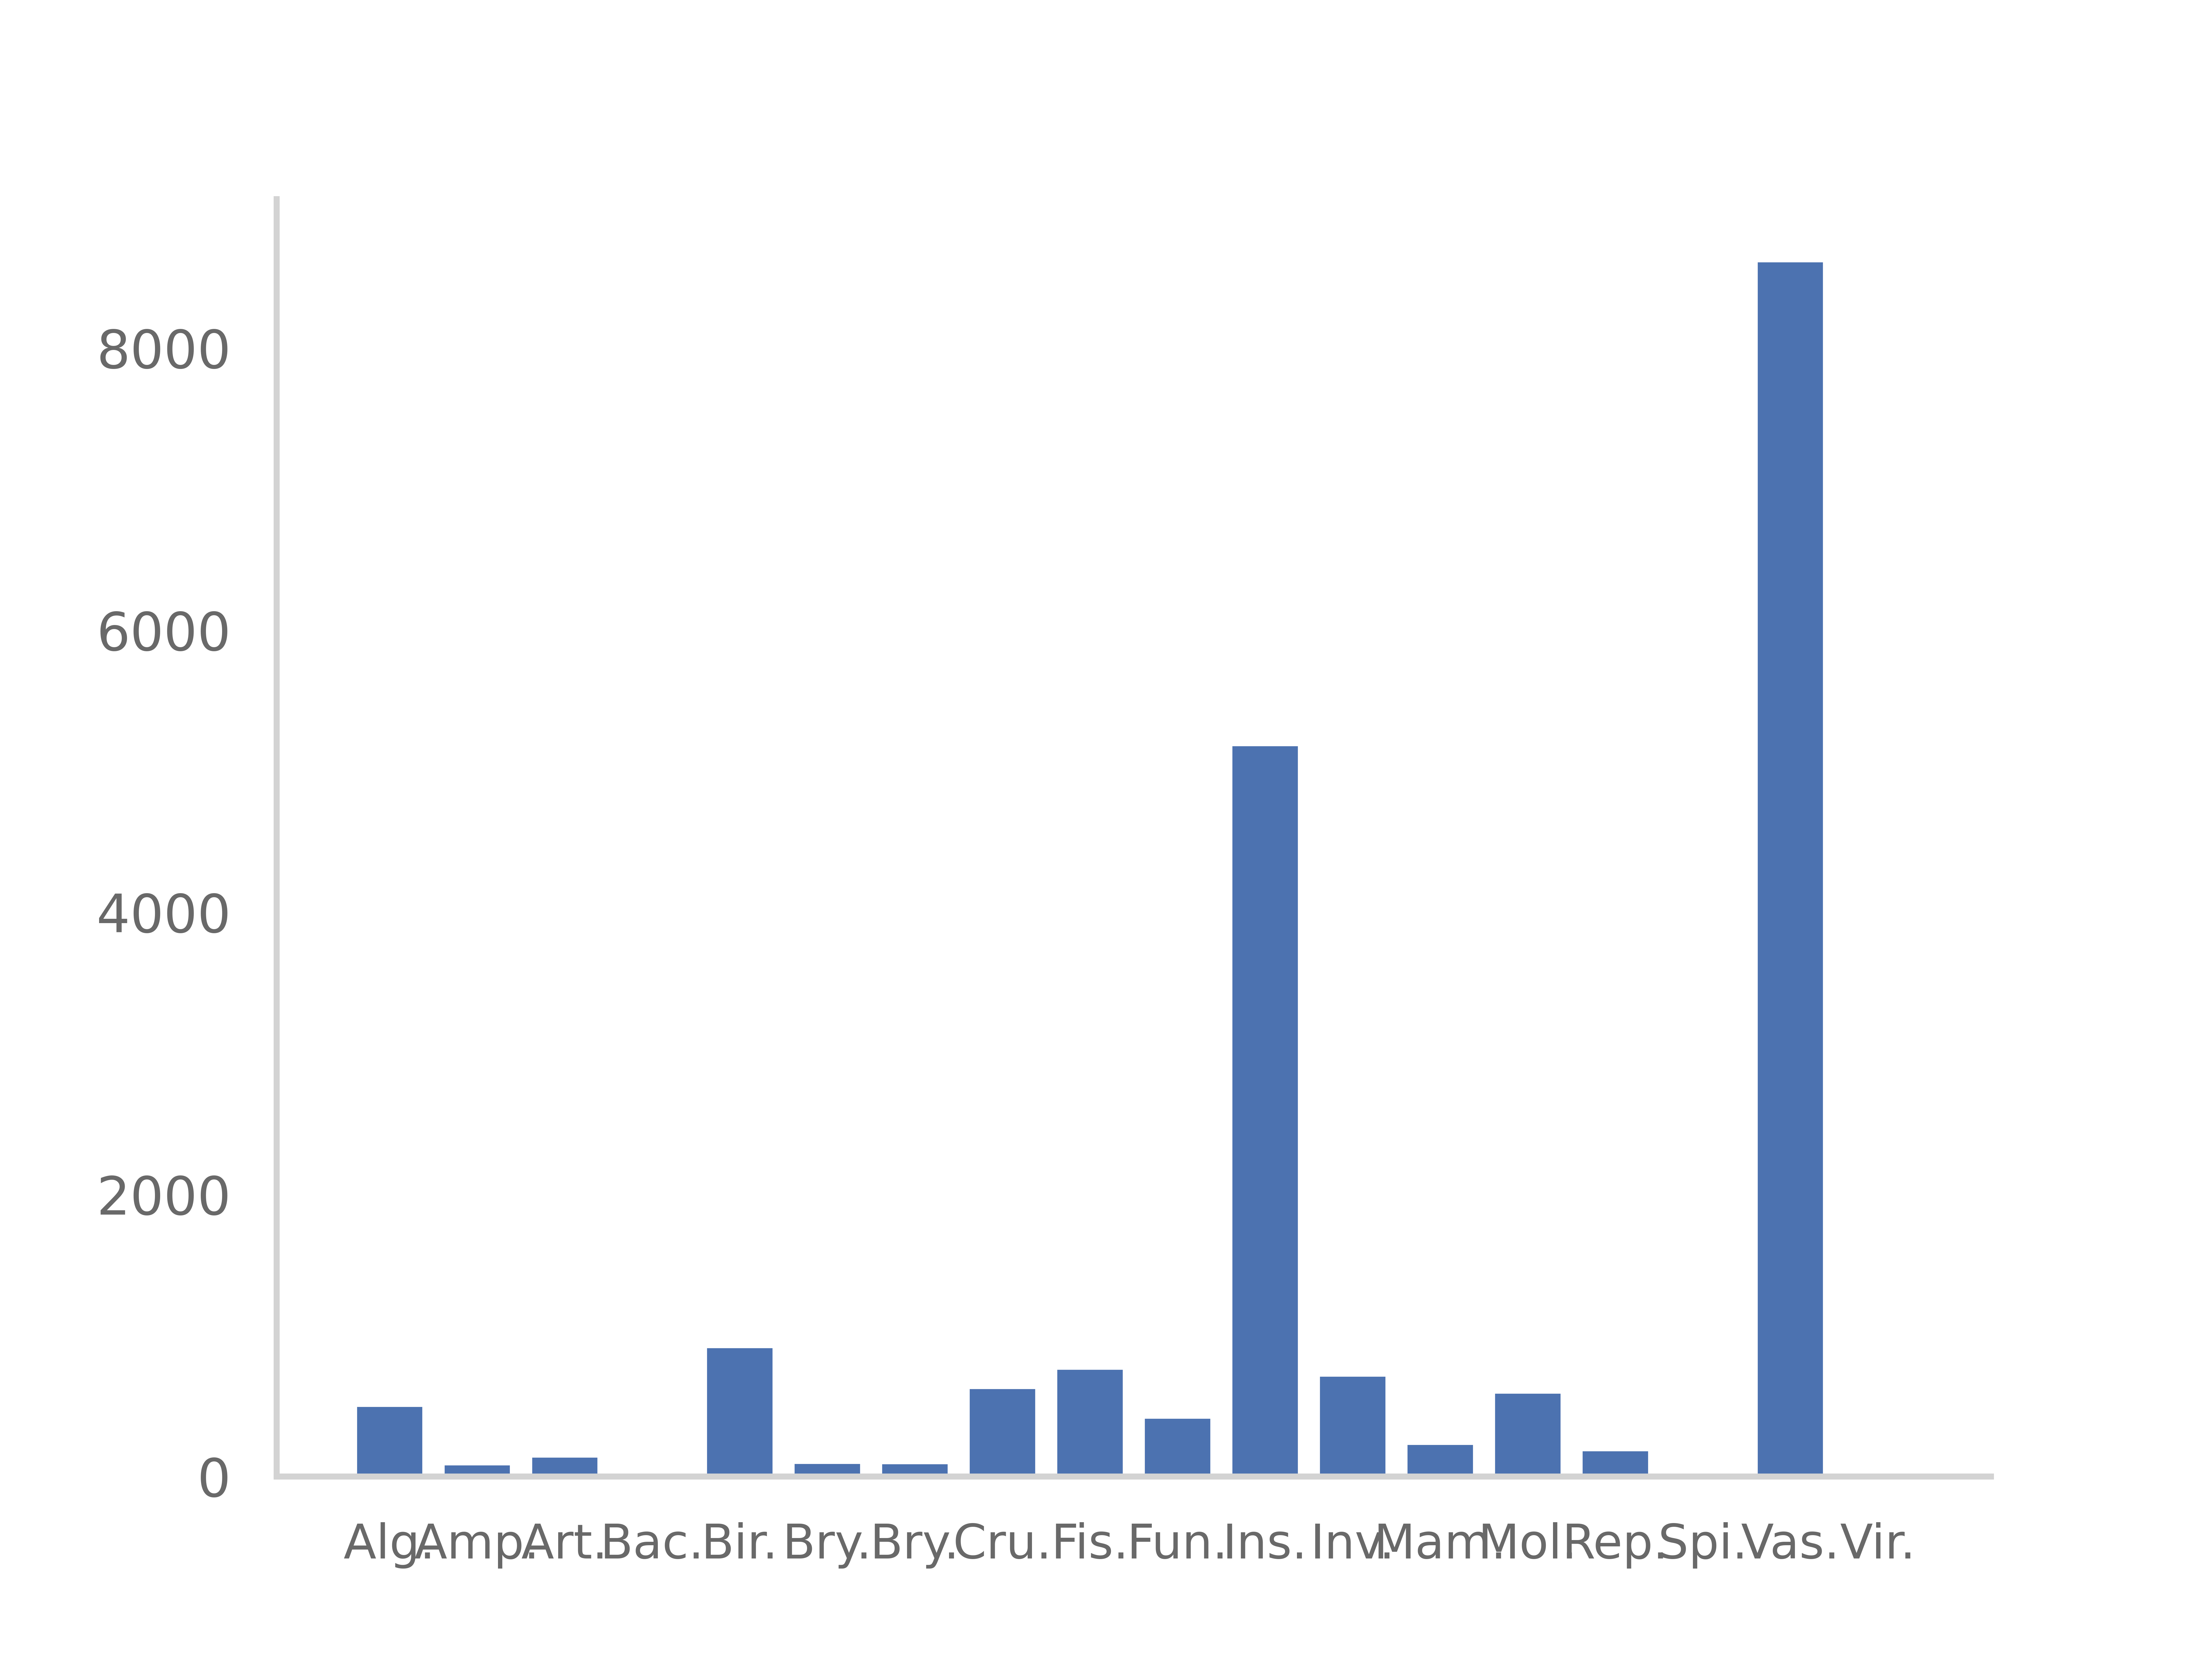
\includegraphics[width=0.9\textwidth]{histogram_taxfam}
    \caption{Histogram of Taxonomic Families \\ and their respective number of species.}
    \label{fig:hist_tax_fam}
\end{minipage}%
\begin{minipage}{.55\textwidth}
    \centering
    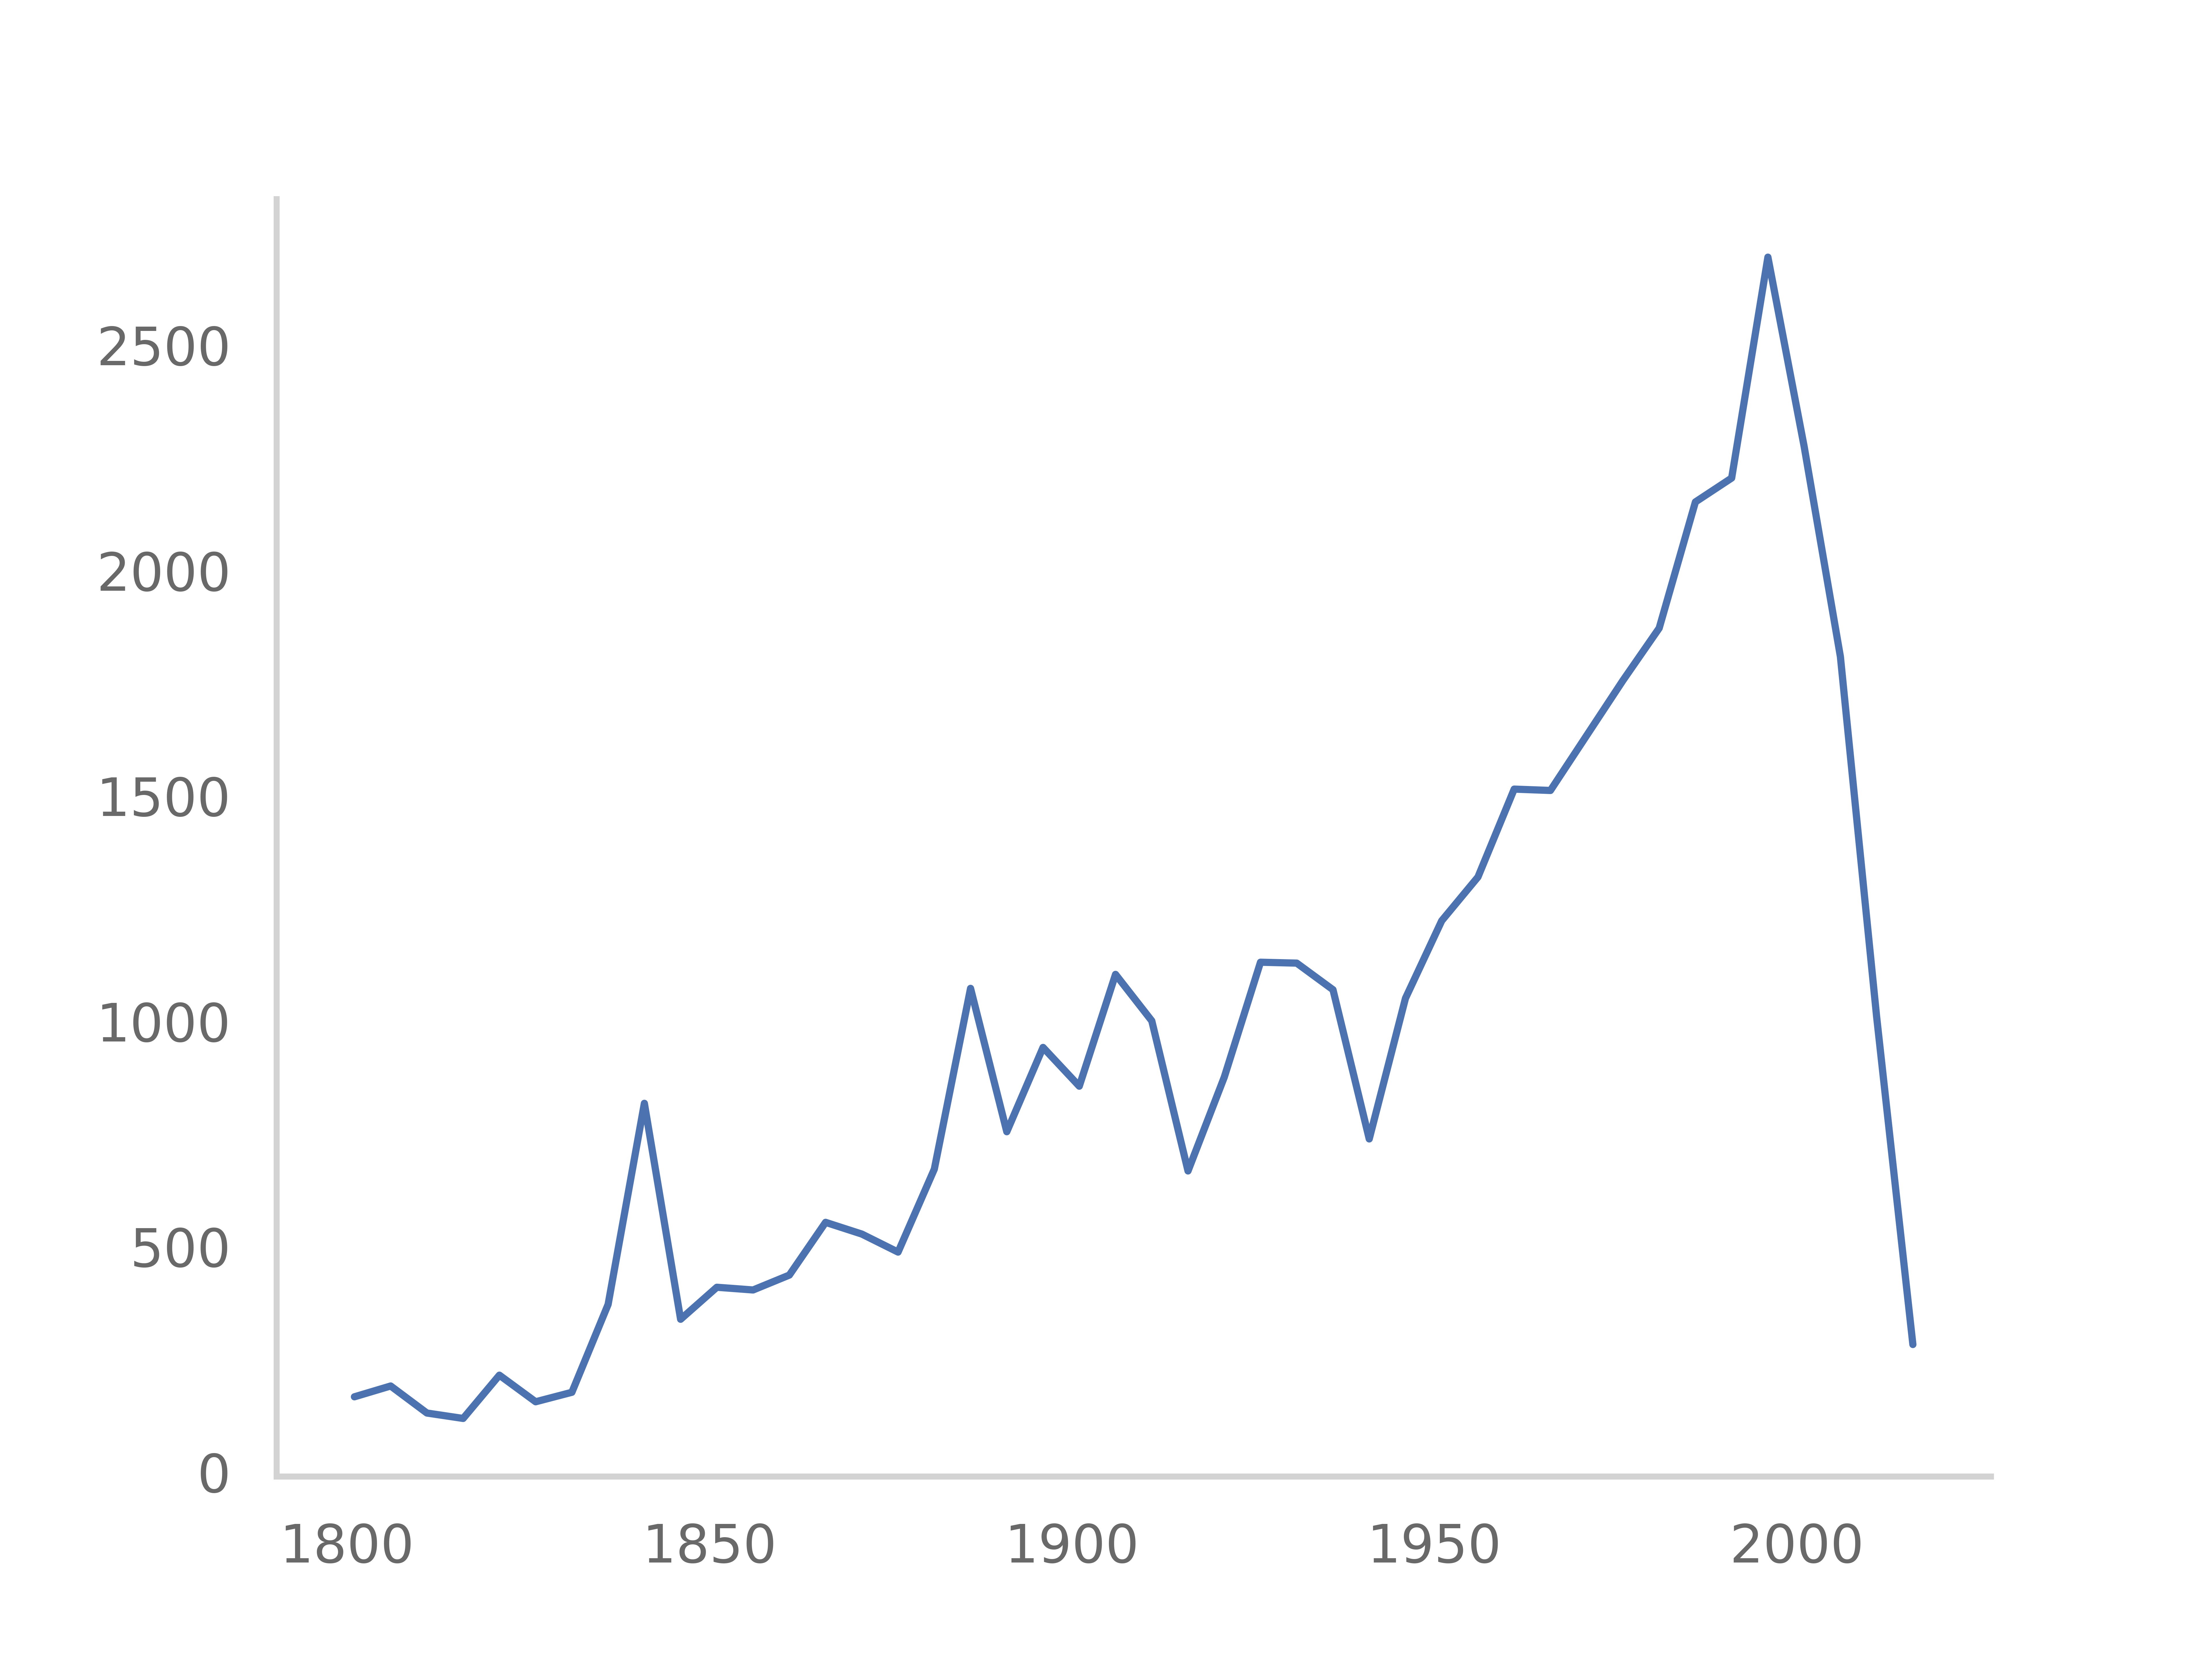
\includegraphics[width=0.9\textwidth]{invasion_per_year.png}
    \caption{Number of invasion per year from 1800 to 2020.}
    \label{fig:invasion_per_year}
\end{minipage}
\end{figure}

Intuitively, the amount invasion per year increases during time mainly due to worldwide effects such as the grow of intercontinental trading and an increased worldwide connectivity (\cite{intro:ecological}). 
%TODO this would be a really good moment to add some insights from the lady

This claim is indeed supported by the dataset, in fact looking at Fig. \ref{fig:invasion_per_year} the number of invasion per year from 1800 to 2020 is monotonically increasing. The high spike after 2000 should not be trusted because the dataset is being constantly updated and recent data may still be lacking. We hence decided to sample the dataset from 1850 to 2010 to ensure reliability and trustiness of the data.

\begin{figure}[H]
    \centering
    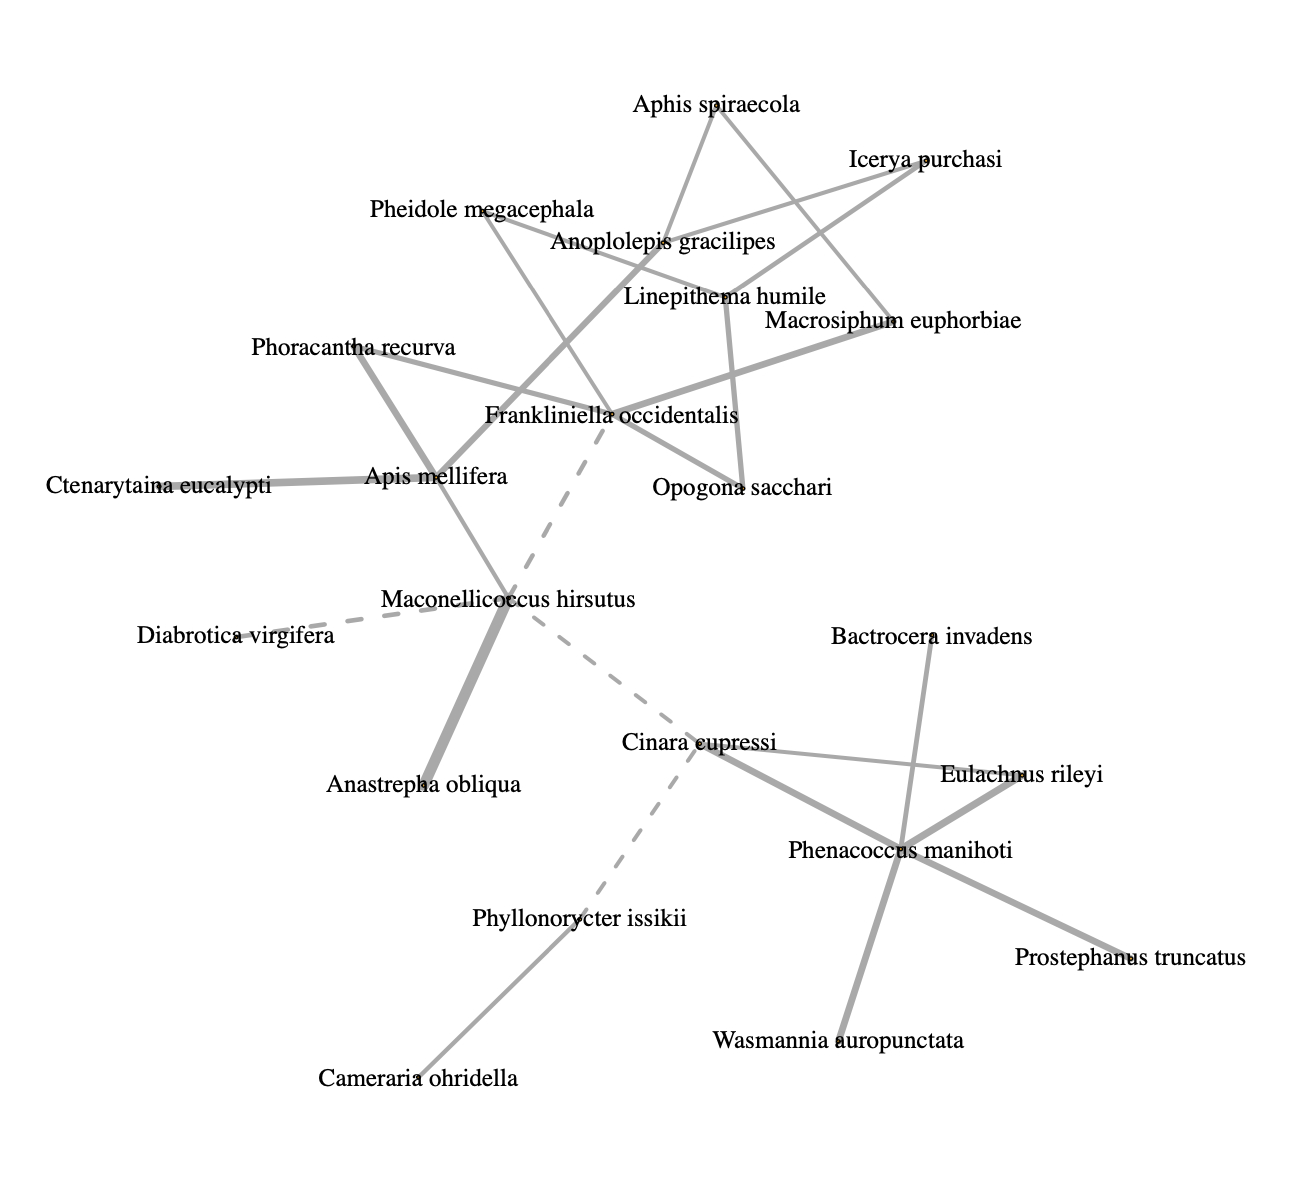
\includegraphics[width=0.75\textwidth]{coinvasion.png}
    \caption{Symmetric interactions between insects in co-invading events. Each node represents a species and the edge represents the strength of the co-invasion factor. A thick edge indicates that a spread of one of the two species in the relationship is tipically followed by the invasion of the second. Image gently taken from \cite{intro:ecological}}
    \label{fig:hist_tax_fam}
\end{figure}

The peak number of invasion per year is around 2500 invasions happened around 2000. Taking into the consideration the large size of the dataset (more than 50'000 species) the number of invasion per year is really low and the dataset is hence considered sparse. The two probability density functions (PFF) in Fig. \ref{fig:pdf_invasion} shows in a very convenient way the sparsity of the dataset. The average number of region invasion per species is 4, this means each species only invaded 4 regions out of the 276 in the entire timeframe of the dataset. The distribution is in fact largely skewed with a standard deviation of 5. It's worth mentioning that the maximum number of invasions is 97 with one outsider that invaded 176 regions. 
%TODO who is this outsider?

Due to the high sparsity of the dataset and the large computational cost of our method, we made a couple of assumptions. The first assumptions is that islands are do not significantely contribuite to the diffusion of species. The second assumption is that any species and region with a low number of invasions is not relevant to our study. Under these two assumptions, we removed %TODO

%%Info right after removing islands
%There are 18 families and 153 regions
%There are 15947 species.
%TODO add a better claim for this assumption

%TODO I removed the region-species PDF
 removed all the species that did not invade a significant amount of regions and all the regions that were not invaded by a significant number of species with the goal of reducing the memory requirements to store the species-region interaction matrix. Fig. \ref{fig:pdf_invasion} shows how the majority of species invaded only a few number of regions. We make the assumption that a any species not invading at least 15 regions out of 276 has no relevant contribution to the model. With these restrictions the dataset has been reduced from 20473 species and 276 regions (55451 invasions in total) to 446 species and 238 regions (10275 invasions in total) number of invasions which is computationally manageable. 

\begin{figure}
\centering
\begin{minipage}{.5\textwidth}
  \centering
    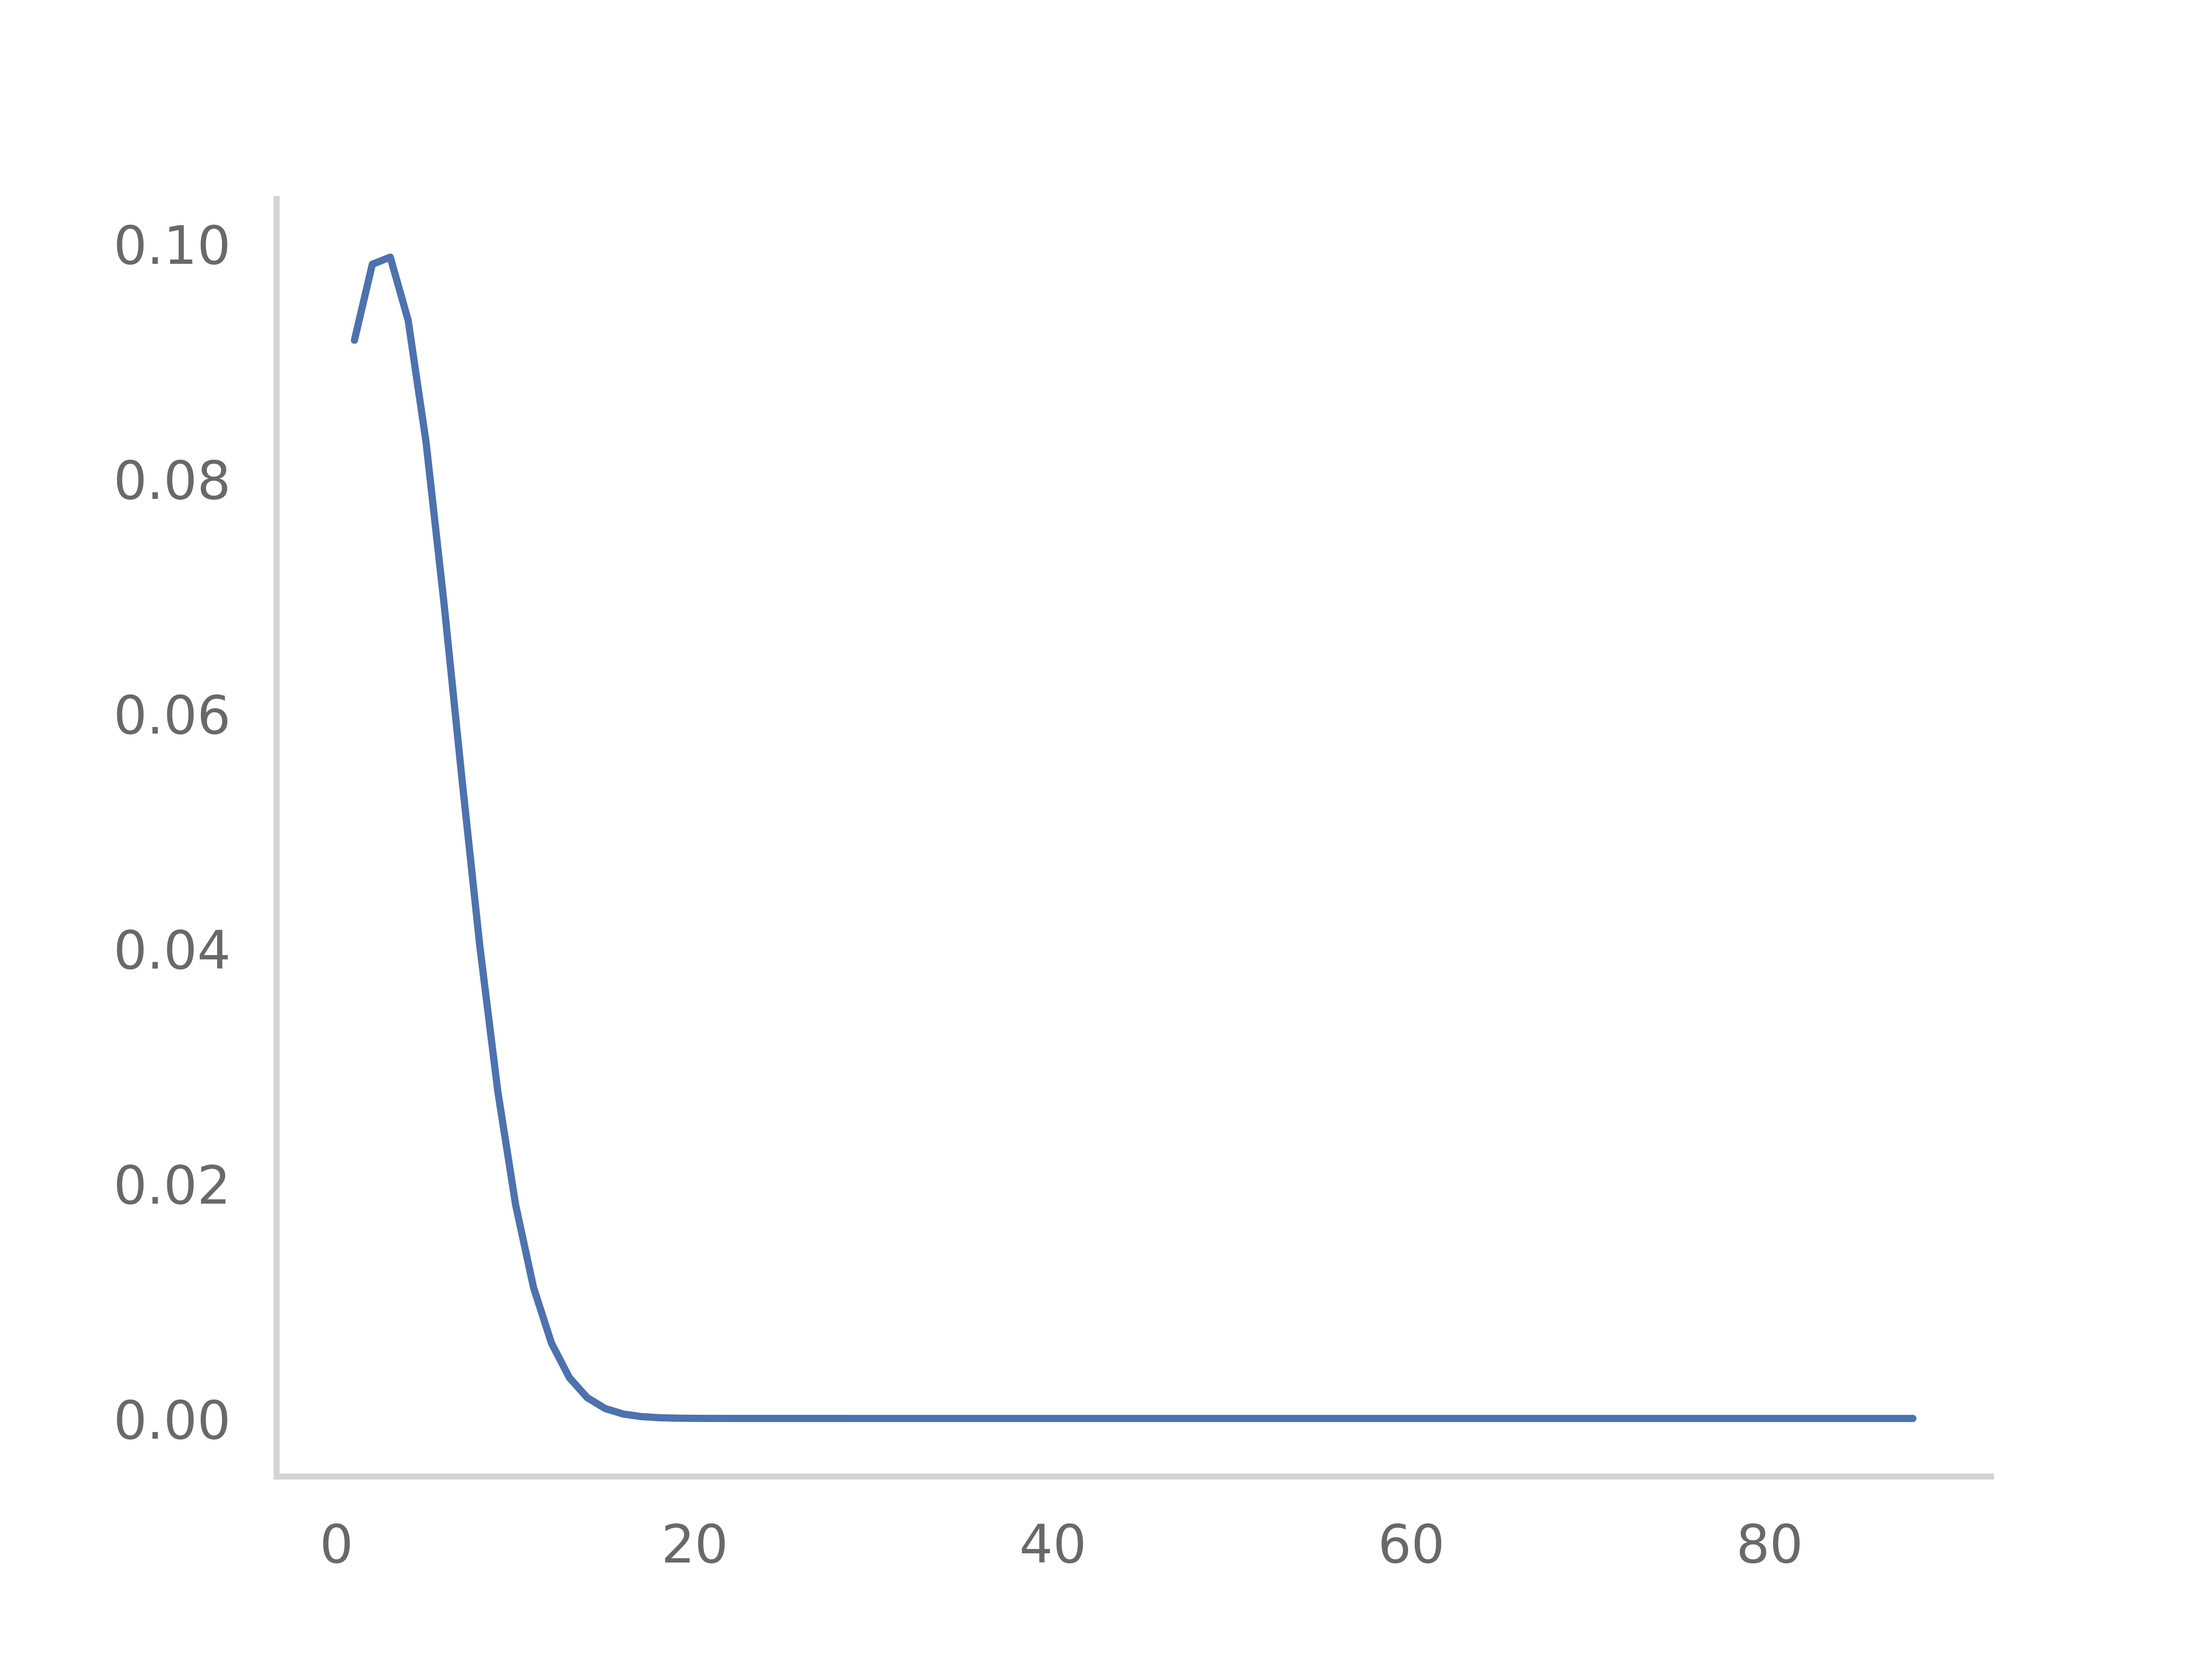
\includegraphics[width=0.85\textwidth]{species_region_invasion_no_filter.png}
%    \caption{Probability density function of of the number of invasions.}
%    \label{fig:pdf_invasion_filtered}
\end{minipage}%
\begin{minipage}{.5\textwidth}
  \centering
    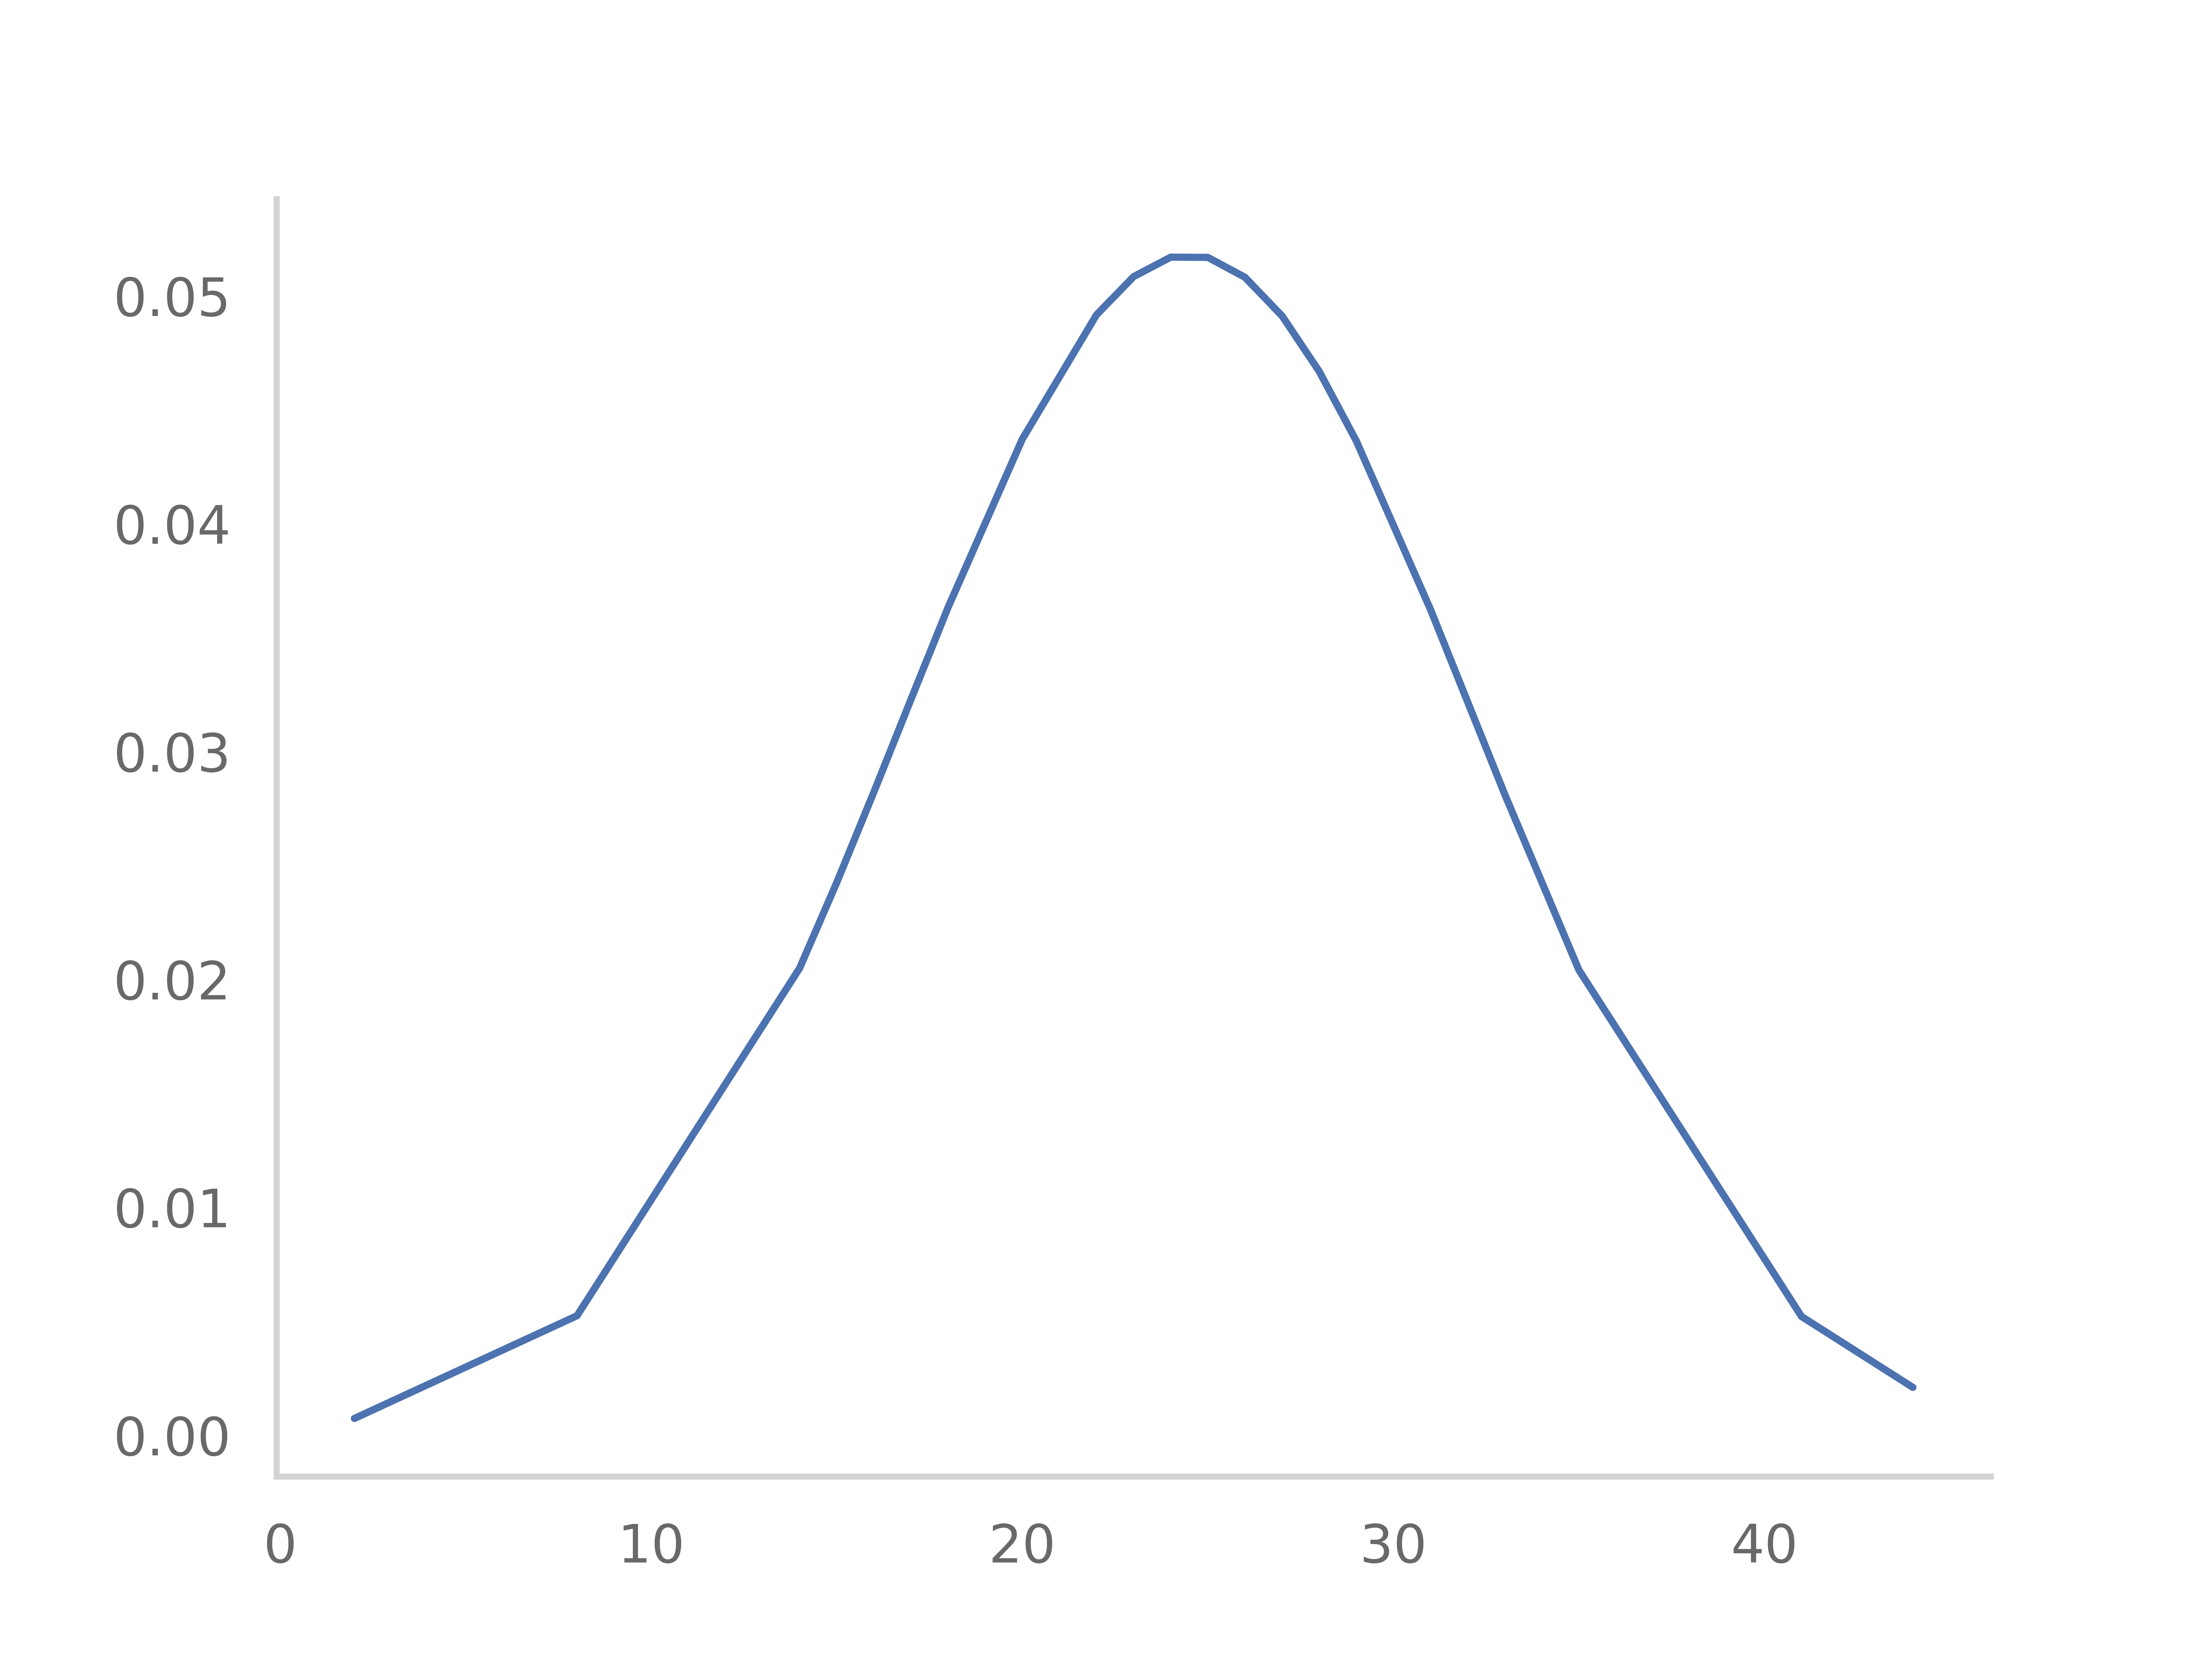
\includegraphics[width=0.85\textwidth]{species_region_invasion.png}
%    \caption{Probability density function of of the number of invasions.}
\end{minipage}

\caption{Probability density function (PDF) of the number of invasions during the entire time frame of the study (1850-2010). The left graph shows that the PDF is strongly left skewed. The second PDF, on the right, is generated after removing all species that did not invade a significant amount of regions.}
\label{fig:pdf_invasion}
\end{figure}

%TODO fix the citation of the lady's paper
\citet{paper:lady} showed that 
%TODO rephrase this
%The effect of distance on the invasion rate (i.e. recording in anew regions) has grown over time, with the rate of invasion events (i.e. the instantaneous rate at which the invasion event occurs among other possible invasions) decreasing with distance to the closest invaded region (Figure 1a). This relationship became especially strong after 1980 for mammals and in- sects.

\chapter{Literature background}

In this section, we cover all the necessary background tools to develop our latent space relational event model. First, we introduce the concept of a latent space model by means of a state space model. Then we cover in-depth the relational event model framework. We introduce then the reader to the Expectation-Maximization and Kalman Filter algorithms. 

\section{State space model}
\label{sec:latent_space}
%http://www.scholarpedia.org/article/State_space_model

\begin{figure}[H]
    \centering
    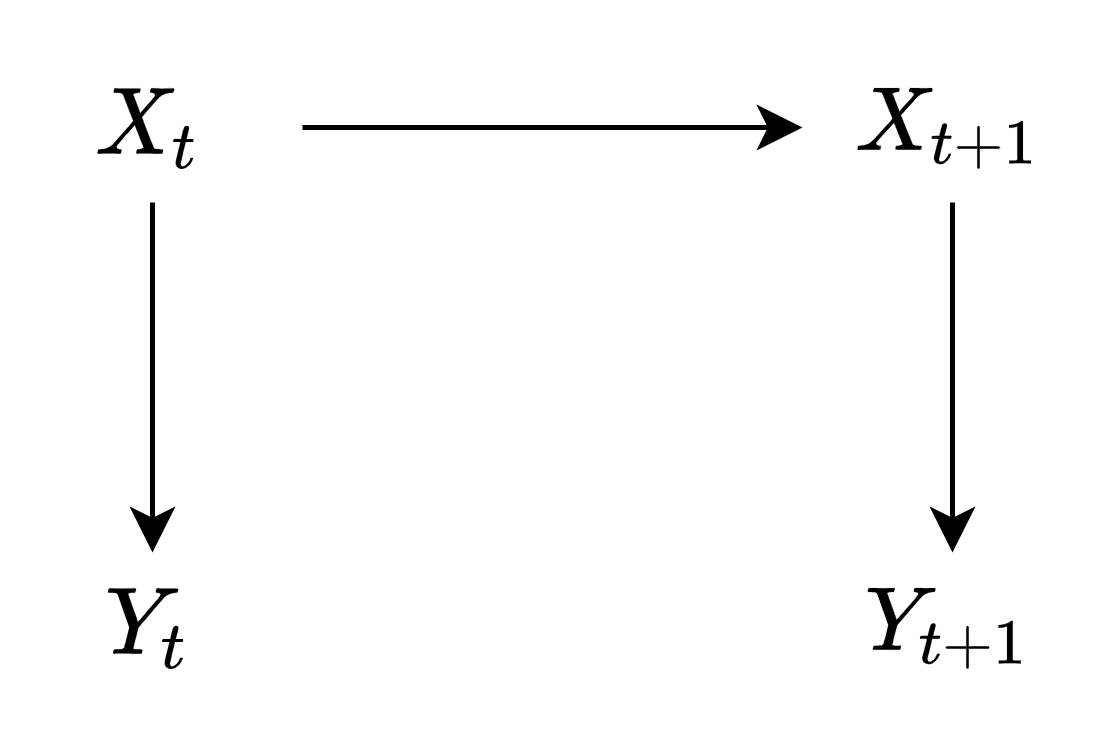
\includegraphics[width=0.35\textwidth]{statespace_diagram.png}
    \caption{State space model diagram representation.}
    \label{fig:pdf_invasion}
\end{figure}

A state-space model is a class of temporal probabilistic models that describe the statistical dependency of latent variables and observed measurement, respectively in the state space $X \in R^d$ and the observed space $Y \in R^m$. In the simplest state-space model, the dynamics are assumed to be a random walk where the jumps between two-time intervals are affected by noise. The first example of such models is the linear Gaussian state-space model, given as follows

\begin{eqfloat}
\begin{equation}
    \begin{cases}
      x_k = A x_{k-1} + \epsilon \; , \quad \epsilon ~ N(0, \Sigma_1) \\
      y_k = B x_k + \delta  \; , \quad \delta ~ N(0, \Sigma_2)  \\
      \textrm{for} \; k = [0, ..., n]
    \end{cases}\,.
\label{eq:statespace}
\end{equation}
\caption{State space model}
\end{eqfloat}

where the matrix $A \in R^{dxd}$ is the state-transition matrix where $d$ is the dimensionality of the state space $X$. Similarly, $B \in R^{mxm}$ is the observation-transition matrix where $m$ is the dimensionality of the observation space $Y$. The linear Gaussian model can be extended in various ways. In our study, we consider a special case of state-space models.

\section{Relational event models (REM)}
\label{background:rem}

\citet{rem:butts} proposed a statistical modeling framework capable of analyzing temporal information and the evolution of a sequence of relational events. Given a set of receiver nodes, a set of sender nodes, and a timeframe, a relational event $e$ is a triplet of a sender, a receiver, and a timestamp. Depending on the underlying data, the sender set and receiver set may be the same set or disjoint sets, depending on the kind of relationship between senders and receivers. For example, for studying the interaction between domestic animals the sender and receiver nodes belong to the same set \cite{intro:cattle}. In contrast, when studying alien species invasion the species are the senders, the regions the receivers and they belong in disjoint sets. In general, a REM specifies varying distributions for all dyads as a function of past events $E=(e_1, ..., e_N)$ where each event $e_i$ is defined as

\[
e_i = (s_i, r_i, t_i)
\]

In the above notation, $s_i \in S_{t} $ is a sender node, $r_i \in R_{t}$ a receiver node and $t_i$ is the time of the interaction. The sets $S_i, R_i$ respectively contain the receiver and senders nodes.

% The cross product of these two sets is called \textit{risk set} $R_{t_i}$  \footnote{\label{riskset_footnote}To avoid confusion, note that Butts originally called this set the \textit{support set}.}
%
%\[
%R_{t_i} = S_{t_i} \times R_{t_i}
%\]

The risk set $\mathcal{R}_t$ is the set of all dyads for which, at a given timestamp $t$, a relational event can occur.

\[
\mathcal{R}_{t} = \{(s,r) \; | \; \textrm{may occurs} \; \textrm{at} \; t_i\}
\]

The waiting time $T_{s,r}$ for a particular dyad to happen between a species $s$ and a region $r$ is assumed to be exponentially distributed 

\[
T_{s,r} \sim Exp(\lambda(s, r, t)
\]


In the above equation, the hazard function $\lambda$ is defined as

\[
\lambda(s, r, t) = \lim_{\delta t \lim 0^+} \frac{P(t \leq T_{s,r} \leq t + \delta t | t \leq T_{s,r})}{\delta t}
\]

The hazard function can be interpreted as the expected number of relational events in a time interval of length one, conditionally on the previous network events. The most commonly used hazard function is the Cox proportional hazard model. 

%%Theta is what thet called beta in Igor's paper (change it?)

\[
\lambda(s, r, t) = \lambda_0(t) \cdot exp({X_{sr}^{(t)} \beta} )
\]

In this equation, $\lambda_0$ represents a baseline hazard for all dyads in the risk $\mathcal{R}$. Instead, the variable $X_{sr}^{(t)}$ is some dyadic covariate at time $t$. To estimate the parameters $\beta$ we maximize the partial likelihood of the Cox proportional hazard model 


\[
L(\beta) =  \prod_{i=1}^n \frac{exp (X_{s_i r_i}^{(t_i)} \beta) }{ \sum_{(s,r) \in \mathcal{R}_{t_i}} exp({X_{sr}^{(t_i)} \beta} )}
\]

Typically the research interest is to estimate the factors that increase, or decrease, the likelihood $L$, more specifically, the parameter $\beta$.


\section{Expectation Maximization}
\label{sec:em}

The expectation-Maximization (EM) , introduced in 1977 by \citet{paper:dempster}, is a family of algorithms that iteratively cycles between two functions until convergence is satisfied. In doing so, it first computes the conditional expectation of the complete likelihood and then maximizes it. This approach is really powerful when applied to problems in which a direct calculation of the likelihood $p(y|\theta)$ is computationally unfeasible. Furthermore, we are in particular interested in the application of this family of algorithms to problems where the full data is not available or some variables are latent (see Sec. \ref{sec:latent_space}). \\

The expectation procedure (E-step) computes the expectation of the logarithm of the complete data likelihood $Q$

\[
Q(\theta^{(k)}) = E_{x} \left[ log(p(x, y | \theta^{(k)}) \right]
\]

then, with the updated parameter $\theta^{(k)}$ we maximizise $Q$ (M-step) and obtain $\theta^{(k+1)}$. The procedure is illustrated in Fig. \ref{em:cycle}. 

\begin{algorithm}[h]
\While{not converged}{
  $\textrm{E-step:} \;  E[Q(\theta^{(k)})] $\;
 $\textrm{M-step:} \; \theta^{(k+1)} = \textrm{argmax}_{\theta} \; Q(\theta)$
}
  \label{em:cycle}
  \caption{A general Expectation Maximization framework.}
\end{algorithm}

The expectation $E[Q(\theta^n)]$ is typically computationally untractable. Furthermore, its complexity increases with the amount of data fed to the model. There are many approaches available to estimate this quantity \cite{book:EMBook}. In this paper, we are interested in an approach to calculate $Q$ called the Kalman Filter.

% ----------------------------------------------------
%TODO more in detail??
%\begin{eqfloat}
%\begin{equation}
%Q(\theta^n) = E_{\theta^n} \left( log(p(x, y | \theta) \right)
%\label{eq:em_expectation}
%\end{equation}
%\caption{Euclidean distance and dot product}
%\end{eqfloat}
%
%
%\begin{eqfloat}
%\begin{equation}
%Q(\theta^n) = E_{\theta^n} \left( log(p(x, y | \theta) \right)
%\label{eq:em_maximization}
%\end{equation}
%\caption{Euclidean distance and dot product}
%\end{eqfloat}


%The key idea of the EM algorithm is that instead of computing the marginal likelihood (which is computationally unfeasible) we compute a lower bound of it. 
%
%\[
%log p(y_{0:T} | \theta) \geq F[q(x_{0:T}, \theta] 
%\]
%
%where $p(y_{0:T} | \theta)$ is the marginal distribution, $q$ is an arbitrary density function and $F$ is a functional defined as TODO. By iteratively maxising the right hand of the equation we can maximise the left hand (i.e. the marginal distribution).  
%
%Given the latent space model in Eq. \ref{eq:latentspace}, a straightforward way to treat the unknown parameter $\theta \in R^d$ would  be to write the full posterior distribution. Unfortunately, this approach is not feasible.
%
%\[
%p(x_{0:T}, \theta | y_{0:T}) = \frac{p(y_{0:T} | x_{0:T}, \theta) p(x_{0:T} | \theta) p(\theta)}{p(y_{0:T})}
%\]


%There exist many other parameter estimation methods for state space models and for more general statistical models, but here we concentrate on these, because these approaches are the most widely used (probabilistic methods) in the state space context.
% ----------------------------------------------------

\section{Kalman Filter}
\label{sec:kalman}

In 1960 R.E. Kalman published his paper describing a recursive solution to the discrete-data linear filtering problem (\citet{paper:kalmanfilter}). Since then, the Kalman filter gained extreme popularity in the machine learning and robotics research field, particularly in the area of autonomous navigation systems. The Kalman filter estimates the evolution of a process by using feedback control. The filter first computes an estimation of the current process state at some time, then, tries to "filter out" the measurement noise in an iterative process. As such, the Kalman filter equations can be subdivided into two categories: the prediction step and the update step. The prediction step is responsible for projecting forward in time the current state of the system. The update step takes the a-prior estimate given from the prediction step and by taking new measurements of the error tries to obtain an improved a-posterior estimate of the state. Indeed, the general form of the algorithm resembles a predictor-corrector algorithm for solving numerical problems. In this chapter, a brief non-technical overview of the Kalman filter is provided. A reader interested in a more in-depth discussion of the formulation of the Kalman filter is advised to read \citet{paper:Maybeck79}.

%A very “friendly” introduction to the
%general idea of the Kalman filter can be found in Chapter 1 of [Maybeck79], while a more complete
%introductory discussion can be found in [Sorenson70], which also contains some interesting
%historical narrative. More extensive references include [Gelb74], [Maybeck79], [Lewis86],
%[Brown92], and [Jacobs93].

\begin{figure}[h]
    \centering
    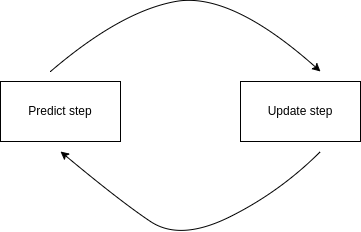
\includegraphics[width=0.25\textwidth]{kalman_diagram.png}
    \caption{The Kalman filter cycle. The time update forwards the current state estimate in time. The measurement update filters the noise out of the projected estimate.}
    \label{fig:kalman_cycle}
\end{figure}

Let's consider the general problem of trying to estimate the configuration of the state $x \in \mathcal{R}^n$ of a linear process evolution in discrete time

\[
x_k = A x_{k-1} + v \; , \quad v ~ N(0, \Sigma)
\]

with a measurement $y_k \in \mathcal{R}^m$ 

\[
y_k = H_k x_k + w \; , \quad w  ~ N(0, \delta) \\
\]

The normal distributed random variables $v, w$ represent noises in the process and in the observation, respectively, and are assumed to be conditionally independent of each other. The matrix $A \in \mathcal{R}^{n, n}$ forwards the state $x_{k-1}$ to the next state $x_k$. The matrix $H \in \mathcal{R}^{m,n}$ relates the measurement $y$ to the process $x$.

The initial state $x_0$ is a random vector with a known mean and variance.

\begin{eqfloat}
\begin{equation}
\begin{array}{l}
\hat{x}_0 = \mu_0 = E[x_0] \\
\hat{V}_0 = V_0 = E[(x_0-\hat{x}_0)(x_0-\hat{x}_0)^T] 
\end{array}
\label{eq:linear_kalman_init}
\end{equation}
\caption{Initialization}
\end{eqfloat}


We define $\hat{x}_k^-$ to be our a-priori estimate of the state $x$ at time $k$, given the knowledge of the previous state. Similarly, we define $\hat{x}_k$ to be our a-posteriori estimate at time $k$ given a measurement $y_k$. The goal of the Kalman filter is to express the a-posteriori state $\hat{x}_k^-$ in terms of a linear combination of the a-priori state and the difference between an actual measurement $y$ and a measurement prediction $H(\hat{x}_k^-)$ state. 


\[
\hat{x}_k = H\hat{x}_k^- + K (y_k - H_k \hat{x}_k^-)
\]
\[
V_k = (I-K_k H_k)V_k^-
\]


For a statistical motivation, I redirect the reader to \citet{paper:Maybeck79}. The difference $y_t - h_t(\hat{x}_t^-)$ is a residual of the estimation against the measurement, reflecting the error between the predicted measurement and the real measurement. The matrix $K$ is called the Kalman gain matrix and is defined as 


\[
K_k = V_k^- H^T_k (H_k V_k^- H^T_k + R_k)^{-1}  \quad , \; H_k = \frac{d}{dx} h(x)
\]


The Kalman gain matrix goal is to minimize the a-posteriori covariance error matrix $V_t$ at time $t$. With some ease, a way of thinking $K$ is that as the measurement error covariance $R$ is close to zero the measurement $y$ is trusted more and the update is made with high precision. On contrary, if the a-priori estimate error covariance $P^-$ is close to zero, the actual measurement $y$ is less trusted and the predicted measurement $H\hat{x}_t^-$ trust is increased. The "trust" is then reflected in the weights of the Kalman gain matrix $K$.

We forecast an update of the estimation of $\hat{x} \approx x$ in time

\begin{eqfloat}[H]
\begin{equation}
\begin{array}{l}
\hat{x}_k^- = A_k \hat{x}_k  \\
\hat{V}_k^- = A_k \hat{V}_k^- A_k^T + \Sigma_k \\
\end{array}
\label{eq:kalman_predict}
\end{equation}
\caption{Prediction step}
\label{eq:linear_kalmann_prediction}
\end{eqfloat}

Where $\Sigma_{t}$ the process noise covariance matrix. Then, on the update step, we filter the noise out of the predicted step a priori estimate and obtain a new estimate $\hat{x}_k$

\begin{eqfloat}[H]
\begin{equation}
\begin{array}{l}
K_k = V_k^- H^T_k (H_k V_k^- H^T_k + R_k)^{-1} \\
\hat{x}_k = x_k^- + K (y_k - h(\hat{x}_k^-)) \\
V_k = (I-K_k H_k)V_k^-
\end{array}
\label{eq:kalman_update}
\end{equation}
\caption{Update step}
\label{eq:linear_kalmann_update}
\end{eqfloat}

The choice of $\Sigma$ is not much deterministic. In a practical way, the noise source $\Sigma$ is often used to capture uncertainity in the process model. Hence, a poor model choice can suffice by simply chosing a large enough uncertainity, by selecting a large covariance $\Sigma$. 


%\begin{eqfloat}
%\begin{equation}
%    \begin{cases}
%      x_k = A x_{k-1} + v \; , \quad v ~ N(0, \Sigma) \\
%      y_k = H_k x_k + w \; , \quad w  ~ N(0, \Sigma) \\
%      \end{cases}\,.
%\label{eq:latentspace}
%\end{equation}
%\caption{Latent space}
%\end{eqfloat}


\chapter{Model}

In this section we introduce our custom latent space relational event model. We first define what the relational events are in our study, the structure of the latent space and how to infer on it. Our study is based on the Alien Species First Records database \cite{intro:dataset} as processed in the previous section.

\section{Latent space relational event model}


%TODO move to model section + note that in our case the matrix A is eye
Given a relation event model with $p$ actors, we define a vector space $V$ where each actor is a vector and the position of each vector is constrained by the distance to all the other vectors inside $V$. The distance in this space represents an affinity of each actor (i.e. vector) $i$ to create a connection to another actor $j$ in the relational event model.


\begin{eqfloat}
\begin{equation}
    \begin{cases}
      x_k = x_{k-1} + \epsilon \; , \quad \epsilon ~ N(0, \Sigma) \\
      y_k \approx Poi(\lambda_k) \; , \quad \lambda^{s, r, k} = exp\left(\alpha-dist(x_s(k), x_r(k)) \cdot \lambda_1(k) \right) \\
      \textrm{for} \; k = [0, ..., n]
    \end{cases}\,.
\label{eq:latentspace}
\end{equation}
\caption{Latent space}
\end{eqfloat}

Distances between vectors are defined in many different ways. Two main popular choices are euclidean distance and dot product. These two distances give a different interpretation to the model. Using the Euclidean distance will impose a symmetric interpretation, in contrast, using a dot product distance will impose an asymmetric interpretation.

\begin{eqfloat}
\begin{equation}
\begin{array}{l}
dist_{euc}(x, v) = |\sum_{i=0}^d x_i - v_i|^2 \\
dist_{dot}(x, x) = x \cdot v
\end{array}
\label{eq:distance_latentspace}
\end{equation}
\caption{Euclidean distance and dot product}
\end{eqfloat}

Generally speaking, the main interest in studying a state-space model is to infer the state configuration $X$ and the rate function $\lambda$ based on temporal observation.
%----------------------- end latent space

%---- begin REM -------------
%TODO distances between nodes in latent space
%set exponentially distributed as the distance species-region in the latent space. {X_{sr}^{(t)

A relational event is an invasion of a species into a region. This relational event is unidirectional and bipartite. In fact, only a species can invade a region, a region can't invade any other region (or specie), and no species-species (or region-region) relational event is allowed. We dispose the regions and species in a latent space $V$ as explained in Eq. \ref{eq:latentspace}. Without loss of generality, we assume that the relation events happen at discrete time intervals. The dynamics on the latent space can be modelled as a random walk where the lenght of the jumps are dependent on the variance $\Sigma$.

%\begin{eqfloat}[H]
%\begin{equation}
%X_{k} = X_{k-1} + \epsilon \quad \epsilon ~ N(0, \Sigma)
%\label{eq:lambda_likelihood}
%\end{equation}
%\caption{Latent space random walk.}
%\end{eqfloat}


The structure of the latent space $X$ is driven by the similarity between regions and species. We expect species that tend to co-invade the same regions to be close in the latent space. Analogous, regions invaded by the same group of species should be near. We are interested in studying the structure of the latent space $V$ to infer on which group of species has the tendency to co-invade regions.
%TODO talk about the distance of nodes in latent space here


%TODO this is censoring. Is this okay?
Every invasion of a species $s_i \in S$ and region $r_j \in R$, where $S, R$ are respectively the sets of species and regions in the dataset, can be modelled as a multivariate Poisson counting measure $$N_t(s_i, r_j) = count{invasion s_i -> r_j \; in \; interval \; [0, t]}$$ such that $S+R = N$ where $N$ is the total number of actors. However, due to the nature of the dataset, a invasion can happen only once. A species is not allowed to "leave" a region and invade it again later in time. Hence the count process is bounded by 1. We define $T(s_i, r_j)$ to be a function that returns the time of invasion for specie $i$ an region $j$. The function $N$ can either take value 1 or zero depending whether an invasion happened previously to t for a determinated region and species.

\[
N_t(s_i, r_j) = 0 \; if \; t < T(s_i, r_j)
\]
\[
N_t(s_i, r_j) = 1 \; if \; t >= T(s_i, r_j)
\]

The stochastic intensity of the counting process $N$ is modelled by the function $\lambda$. Heuristically, we assume that the rates $\lambda$ are functions of the distance between species and regions in the latent space (Eq. \ref{eq:latentspace}). The distance of the nodes in $X$ is modelled using a dot product, which captures the similarity of actors.

%TODO what about exogenoues/edogeneous effects ?
\begin{eqfloat}
\begin{equation}
\lambda^{s, r, k} = exp\left(\alpha-(x_s(k) \cdot x_r(k)) \cdot \lambda_1(k) \right) \\
\label{eq:ourmodel_lambda}
\end{equation}
\caption{Lambda rates are in function of the distance given by the dot products of vectors in the latent space $X$.}
\end{eqfloat}

To infer on the structure of the latent space $X$, and the parameters $\theta$  and $\Sigma$ we use the Expectation Maximization (EM) algorithm (\ref{sec:em}). Since the latent state $X$ is not observed, a direct optimization of the maximum likelihood is not possible. We aim to maximise the $\int_x L(\theta, \Sigma ; y, x) dx$. As explained in the background section, the EM instead of directly maximise this integral, it iteratively computes an estimate $Q$ of the parameters $\theta, \Sigma$ conditionated on the previous estimate. 

\[
Q(\theta^{n}, \Sigma^{n}) = E_{x|y} \left( log(p(x, y | \theta^{n-1}, \Sigma^{n-1}) \right)
\]

%TODO 
The expectation of the log-likelihood can be estimated using an extended Kalman filter \ref{sec:kalman}. Calculating the entire conditional distribution is computationally unfeasible, therefore, we only calculate the first two moments. We denote $\bar{x}_{k}$ and $\bar{V}_{k}$ as the expectation and variance of the state process $x$ conditioned up to the observed state $y_k$. 



%---------------------------------------------------------------------------------------------------

%TODO review this
% I should mention that our process is not linear,however, we can linearise it and apply an Extended KF
% also mention that only one step is required for convergence

Let's consider a non-linear system, $\epsilon$ captures uncertainty in the model, $v$ denotes the measurement noise. Both variables are white noises, random distributions with zero mean, and uncorrelated. 

%TODO why is this more general?
\[
x_k \sim f(x_{k-1}) + \epsilon_k \; , \; \epsilon ~ N(0, \Sigma)
\]
\[
y_k \sim h(x_{k}) + v_{k} \; , \; v ~ N(0, \Delta)
\]
%
%The initial state $x_0$ is a random vector with a known mean and variance.
%
%\begin{eqfloat}
%\begin{equation}
%\begin{array}{l}
%\hat{x}_0 = \mu_0 = E[x_0] \\
%\hat{V}_0 = V_0 = E[(x_0-\hat{x}_0)(x_0-\hat{x}_0)^T] 
%\end{array}
%\label{eq:kalman_init}
%\end{equation}
%\caption{Initialization}
%\end{eqfloat}

Providing that $f, y \in C^1$, we can linearise the process around the mean. 
%
%We define $\hat{x}_k^-$ to be our a-priori estimate of the state $x$ at time $k$, given the knowledge of the previous state. Similarly, we define $\hat{x}_k$ to be our a-posteriori estimate at time $k$ given a measurement $y_k$. The goal of the Kalman filter is to express the a-posteriori state $\hat{x}_k^-$ in terms of a linear combination of the a-priori state and the difference between an actual measurement $y$ and a measurement prediction $H(\hat{x}_k^-)$ state. 
%
%%\[
%%\hat{x}_t \in span(\hat{x}_t^-, y_t - H\hat{x}_t^-) 
%%\]
%\[
%\hat{x}_k = H\hat{x}_k^- + K (y_k - H_k \hat{x}_k^-)
%\]
%\[
%V_k = (I-K_k H_k)V_k^-
%\]
%
%
%For a statistical motivation, I redirect the reader to \citet{paper:Maybeck79}. The difference $y_t - h_t(\hat{x}_t^-)$ is a residual of the estimation against the measurement, reflecting the error between the predicted measurement and the real measurement. The matrix $K$ is called the Kalman gain matrix and is defined as 
%
%
%\[
%K_k = V_k^- H^T_k (H_k V_k^- H^T_k + R_k)^{-1}  \quad , \; H_k = \frac{d}{dx} h(x)
%\]
%TODO mention that the Kalman matrix here is different

 We forecast an update of the estimation of $\hat{x} \approx x$

\begin{eqfloat}[H]
\begin{equation}
\begin{array}{l}
\hat{x}_t^- = f(\hat{x}_{t-1}) \\
\hat{V}_t^- = J(x^f_{t-1}) V_{t-1} J(x^f_{t-1})^T + W_{t-1} Q_{t-1} W_{t-1}^T
\end{array}
\label{eq:kalman_predict}
\end{equation}
\caption{Prediction step}
\label{eq:kalmann_prediction}
\end{eqfloat}

Where $J(x)$ is the Jacobian of $f(x)$ and $Q_{t-1}$ the process noise covariance matrix.


\begin{eqfloat}[H]
\begin{equation}
\begin{array}{l}
K_t = V_t^- H^T_t (H_t V_t^- H^T_t + R_t)^{-1} \\
\hat{x}_t = x_t^- + K (z_t - h(\hat{x}_t^-)) \\
V_t = (I-K_t H_t)V_t^-
\end{array}
\label{eq:kalman_update}
\end{equation}
\caption{Update step}
\label{eq:kalmann_update}
\end{eqfloat}

Where K is the Kalmann gain. By combining equations (\ref{eq:kalmann_prediction}), (\ref{eq:kalmann_update}) we get an algorithm for the Extended Kalman Filter process is shown in Algorithm \ref{algo:kalmann}. 

\begin{algorithm}[H]
\textbf{Initialize: }
\begin{substeps}
$\hat{x}_0 = \mu_0 = E[x_0]$ \;
$\hat{V}_0 = V_0 = E[(x_0-\hat{x}_0)(x_0-\hat{x}_0)^T]$  \;
\end{substeps}
\For{k=1,...,n}{
  Prediction step (Eq. \ref{eq:kalmann_prediction})
  \begin{substeps}
  $\hat{x}_t^- = f(\hat{x}_{t-1})$ \;
  $\hat{V}_t^- = J(x^f_{t-1}) V_{t-1} J(x^f_{t-1})^T + W_{t-1} Q_{t-1} W_{t-1}^T$\;
  \end{substeps}
  Update step (Eq. \ref{eq:kalmann_update})
  \begin{substeps}
  $K_t = V_t^- H^T_t (H_t V_t^- H^T_t + R_t)^{-1}$ \;
  $\hat{x}_t = x_t^- + K (z_t - h(\hat{x}_t^-))$\;
  $V_t = (I-K_t H_t)V_t^-$\;
  \end{substeps}
}
  \caption{Extended Kalmann Filter}
  \label{algo:kalmann}
\end{algorithm}

%---------------------------------------------------------------------------------------------------


%TODO review my notation in section KF. First two moments
%also seee star at igor paper 3. Inference
\[
\bar{x}_{k} = .... \\
\bar{V}_{k} = ....
\]

By assuming that a step in time in the latent state can be approximated by the conditional distribution 

\[
x_{k-1 | k-1} \approx N(\bar{x_{k-1 | k-1}}, \bar{V_{k-1|k-1}})
\]

the predict step of the Kalman filter estimates the first two moments of $x_k$. 


%For the initial state $k=0$ we set $x_{0|0} = x_0$ and $V_{0|0} = \Sigma_0$ arbitrarly.

%TODO what is this lol?
%Similarly to as explained in Sec. \ref{background:rem}, 
%
%\begin{eqfloat}[H]
%\begin{equation}
%L(\lambda) =  \prod_{e \in E} \frac{\lambda_1(s_i, r_i, t_i | G, \theta)}{ \sum_{s \in R_{t_i}} \lambda_1(s, r, t_i | G, \theta)} + \lambda_0
%\label{eq:lambda_likelihood}
%\end{equation}
%\caption{Full log-likelihood of hazard function.}
%%\label{eq:kalmann_update}
%\end{eqfloat}

\chapter{Discussion}

%TODO our findings are in agreement with lady's paper

%The number of alien species found in a particular region. Both plants and insects were significantly affected by the number of species that have already invaded a certain region. However, whereas plants were recorded more frequently in regions already invaded by other plants, insects were less frequently recorded in regions that had already been invaded by other in- sects. The effects were nonetheless very small in both cases, i.e., affecting the hazard by 0.3% per invasion in the opposite direction.



%TODO move this to appendix or whatever
%\subsection{Implementation specifications}
%We implemented the method discussed in TODO section in Tensorflow (TODO add cite) 
%
%%%TODO what framework do we use - how we solved the computational cost problem
%The size of the dataset is problematic under a computational point of view. In particular, the inversion of the matrix TODO and the memory requirements to allocate all the dataset are large. However, due to the filtering described in the previous section and using efficient data structure by saving in memory only the non-zero entries and the indexes in a sparse matrix and by using CUDA toolokits to accelerate the computation in GPU our implementation meets the computational requirements.
% 
 
 
%-------- useless stuff ? ----------
%\section{The second, math section}
%
%\textbf{Theorem 1 (Residue Theorem).}
%Let $f$ be analytic in the region $G$ except for the isolated singularities $a_1,a_2,\ldots,a_m$. If $\gamma$ is a closed rectifiable curve in $G$ which does not pass through any of the points $a_k$ and if $\gamma\approx 0$ in $G$ then
%\[
%\frac{1}{2\pi i}\int_\gamma f = \sum_{k=1}^m n(\gamma;a_k) \text{Res}(f;a_k).
%\]
%\textbf{Theorem 2 (Maximum Modulus).}
%\emph{Let $G$ be a bounded open set in $\mathbb{C}$ and suppose that $f$ is a continuous function on $G^-$ which is analytic in $G$. Then}
%\[
%\max\{|f(z)|:z\in G^-\}=\max \{|f(z)|:z\in \partial G \}.
%\]
%
%\section[third]{A very very long section, titled ``The third section'', with
%  a rather  short text alternative (third)}
%\lipsum \texttt{Some Test}
%\lstset{language=algebra,linewidth=0.95\linewidth,breaklines=true,numbers=left,
%basicstyle=\ttfamily,numberstyle=\tiny,escapeinside={//*}{\^^M},
%mathescape=true}
%\begin{lstlisting}
%import IntSpec, ItemSpec;
%
%sort cart; //*\label{sort}
%
%constructors //*\label{begin-sig}
%create() $\longrightarrow$ cart;
%insert(cart, item) $\longrightarrow$ cart;
%observers
%amount(cart) $\longrightarrow$ int;
%transformers
%delete(cart, item) $\longrightarrow$ cart; //*\label{end-sig}
%
%axioms //*\label{begin-axioms}
%forall c: cart, i, j: item 
%
%amount(create()) $=$ 0; //*\label{begin-amount}
%amount(insert(c,i)) $=$ amount(c) $+$ price(i); //*\label{end-amount}
%delete(create(),i) $=$ create(); //*\label{begin-delete}
%delete(insert(c,i),j) $=$
%if (i =$\:$= j) c
%else insert(delete(c,j),i); //*\label{end-axioms}
%end
%\end{lstlisting}
%
%As you can easily see from the above listing \citet{bbggs:iet07}
%define something weird based on the BPEL specification
%\citep{bpelspec}.
%\nocite{*}

%\appendix %optional, use only if you have an appendix

%\chapter{Some retarded material}
%\section{It's over\dots}
%\lipsum 
%
%\backmatter


%\chapter{Glossary} %optional

%\bibliographystyle{alpha}
%\bibliographystyle{dcu}
%\bibliographystyle{plainnat}
%\bibliography{biblio}

\bibliographystyle{abbrvnat}
% \bibliographystyle{plain} % We choose the "plain" reference style
\bibliography{biblio} % Entries are in the refs.bib file
%\cleardoublepage
%\theindex %optional, use only if you have an index, must use
	  %\makeindex in the preamble
%\lipsum

\end{document}
